\documentclass[11pt,]{article}
\usepackage[left=1in,top=1in,right=1in,bottom=1in]{geometry}
\newcommand*{\authorfont}{\fontfamily{phv}\selectfont}
\usepackage[]{mathpazo}


  \usepackage[T1]{fontenc}
  \usepackage[utf8]{inputenc}



\usepackage{abstract}
\renewcommand{\abstractname}{}    % clear the title
\renewcommand{\absnamepos}{empty} % originally center

\renewenvironment{abstract}
 {{%
    \setlength{\leftmargin}{0mm}
    \setlength{\rightmargin}{\leftmargin}%
  }%
  \relax}
 {\endlist}

\makeatletter
\def\@maketitle{%
  \newpage
%  \null
%  \vskip 2em%
%  \begin{center}%
  \let \footnote \thanks
    {\fontsize{18}{20}\selectfont\raggedright  \setlength{\parindent}{0pt} \@title \par}%
}
%\fi
\makeatother




\setcounter{secnumdepth}{3}

\usepackage{longtable,booktabs}

\usepackage{graphicx,grffile}
\makeatletter
\def\maxwidth{\ifdim\Gin@nat@width>\linewidth\linewidth\else\Gin@nat@width\fi}
\def\maxheight{\ifdim\Gin@nat@height>\textheight\textheight\else\Gin@nat@height\fi}
\makeatother
% Scale images if necessary, so that they will not overflow the page
% margins by default, and it is still possible to overwrite the defaults
% using explicit options in \includegraphics[width, height, ...]{}
\setkeys{Gin}{width=\maxwidth,height=\maxheight,keepaspectratio}

\title{Asociación y abundancia relativa de especies de la familia Rubiaceae en
la parcela permanente Isla Barro Colorado  }



\author{\Large J. Alberto Meléndez Juan\vspace{0.05in} \newline\normalsize\emph{Universidad Autónoma de Santo Domingo (UASD)}  }


\date{}

\usepackage{titlesec}

\titleformat*{\section}{\normalsize\bfseries}
\titleformat*{\subsection}{\normalsize\itshape}
\titleformat*{\subsubsection}{\normalsize\itshape}
\titleformat*{\paragraph}{\normalsize\itshape}
\titleformat*{\subparagraph}{\normalsize\itshape}

\titlespacing{\section}
{0pt}{36pt}{0pt}
\titlespacing{\subsection}
{0pt}{36pt}{0pt}
\titlespacing{\subsubsection}
{0pt}{36pt}{0pt}





\newtheorem{hypothesis}{Hypothesis}
\usepackage{setspace}

\makeatletter
\@ifpackageloaded{hyperref}{}{%
\ifxetex
  \PassOptionsToPackage{hyphens}{url}\usepackage[setpagesize=false, % page size defined by xetex
              unicode=false, % unicode breaks when used with xetex
              xetex]{hyperref}
\else
  \PassOptionsToPackage{hyphens}{url}\usepackage[unicode=true]{hyperref}
\fi
}

\@ifpackageloaded{color}{
    \PassOptionsToPackage{usenames,dvipsnames}{color}
}{%
    \usepackage[usenames,dvipsnames]{color}
}
\makeatother
\hypersetup{breaklinks=true,
            bookmarks=true,
            pdfauthor={J. Alberto Meléndez Juan (Universidad Autónoma de Santo Domingo (UASD))},
             pdfkeywords = {palabra clave 1, palabra clave 2},  
            pdftitle={Asociación y abundancia relativa de especies de la familia Rubiaceae en
la parcela permanente Isla Barro Colorado},
            colorlinks=true,
            citecolor=blue,
            urlcolor=blue,
            linkcolor=magenta,
            pdfborder={0 0 0}}
\urlstyle{same}  % don't use monospace font for urls

% set default figure placement to htbp
\makeatletter
\def\fps@figure{htbp}
\makeatother

\usepackage{amsmath}

\usepackage{pdflscape} \newcommand{\blandscape}{\begin{landscape}} \newcommand{\elandscape}{\end{landscape}}


% add tightlist ----------
\providecommand{\tightlist}{%
\setlength{\itemsep}{0pt}\setlength{\parskip}{0pt}}

\begin{document}
	
% \pagenumbering{arabic}% resets `page` counter to 1 
%
% \maketitle

{% \usefont{T1}{pnc}{m}{n}
\setlength{\parindent}{0pt}
\thispagestyle{plain}
{\fontsize{18}{20}\selectfont\raggedright 
\maketitle  % title \par  

}

{
   \vskip 13.5pt\relax \normalsize\fontsize{11}{12} 
\textbf{\authorfont J. Alberto Meléndez Juan} \hskip 15pt \emph{\small Universidad Autónoma de Santo Domingo (UASD)}   

}

}








\begin{abstract}

    \hbox{\vrule height .2pt width 39.14pc}

    \vskip 8.5pt % \small 

\noindent Resumen del manuscrito


\vskip 8.5pt \noindent \emph{Keywords}: palabra clave 1, palabra clave 2 \par

    \hbox{\vrule height .2pt width 39.14pc}



\end{abstract}


\vskip 6.5pt


\noindent  \section{Introducción}\label{introducciuxf3n}

Las comunidades vegetales de los bosques neotropicales ejemplifican la
diversidad y complejidad ecológica de la región tropical. El estudio
continuo de su riqueza y abundancia relativa permite identificar las
especies raras, las cuales son más vulnerables a los cambios en su
hábitat y por lo tanto propensas a extinguirse localmente (Volkov,
Banavar, Hubbell, \& Maritan, 2003). Adicionalmente, monitorear la
diversidad como propiedad de las comunidades vivientes resulta de suma
importancia para analizar el efecto que tiene la transformación de los
ecosistemas en las comunidades naturales. Claramente existe entonces la
necesidad de conocer como se encuentran asociadas las especies entre sí
dentro de las comunidades ecológicas para ayudar a comprender los
factores que inciden en su conservación (Moreno, 2001).

La familia Rubiaceae es un importante grupo de plantas vasculares de
distribución cosmopolita con una marcada diversidad en regiones
tropicales y subtropicales (Davis et al., 2009). Muchas de las especies
que componen esta familia se encuentran adaptadas a la vida en la
penúmbra, y prosperan bajo la sombra del dosel selvático. En estas
selvas tropicales, el grado de ordenación y riqueza de las comunidades
que componen el sotobosque dependen en gran medida de interacciónes
entre las distintas especies (Torres-Leite et al., 2019), además de
factores ambientales de su hábitat, ya que muchas de estas especies
estan adaptadas a rangos elevados de ácidez y otras condiciones
específicas de los componentes del suelo, como la concentración de
distintos metales (Jansen, Robbrecht, Beeckman, \& Smets, 2000).

Es preciso señalar que trabajos anteriores (Condit et al., 2002) sobre
el bosque tropical panameño y el grado de reemplazo entre especies de
distintas comunidades o diversidad beta, sugieren que la disimilaridad
tiende a aumentar en función de la distancia a la cual se encuentran
separadas en el espacio. Sin embargo, estos trabajos no restan
importancia a la variabilidad del hábitat y se toman en cuenta en este
estudio, ya que un acercamiento inicial a los datos de abundancia de las
distintas especies de Rubiaceae en Barro Colorado arrojó indicios de
posibles patrones acerca de su distribución, y se plantea la posibilidad
de que existan especies con algún grado de asociación respecto a las
variables ambientales que allí imperan.

Aunque la distribución de la abundancia de las especies actualmente es
en buena parte atribuida a los mecanismos que definen a una comunidad en
particular, como la prevalencia de especies dominantes, relativamente
más abundantes en comparación con las especies raras. Las medidas para
la distribución de la abundancia relativa se encuentran sujetas a
interacciones que aún no se conocen del todo, ni en qué grado inciden en
la estructura de la comunidad (Néda, Horvat, Toháti, Derzsi, \& Balogh,
2008).

El presente estudio evalúa la relación entre abundancia relativa de
especies de la familia Rubiaceae y su distribución en una porción de
bosque tropical en la parcela permanente Barro Colorado Island (en lo
adelante BCI), Colón, Panamá. Las parcelas permanentes, como BCI, son
una excelente fuente de datos demográficos y posibilitan el estudio
continuo de la diversidad a nivel local y contribuyen a medir el aporte
de la familia Rubiaceae a la diversidad de su comunidad. En ese sentido,
este trabajo aprovecha la información disponible (Hubbell, Condit, \&
Foster, 2021), y herramientas de libre acceso (Martínez Batlle, 2020),
para conocer posibles patrones de asociación entre estas especies, como
varía la diversidad con respecto a las características del hábitat en el
cual crecen estas poblaciones de plantas, y otras condiciones
ambientales mediante análisis estadístico de datos de los censos
realizados en BCI.

\section{Metodología}\label{metodologuxeda}

\subsection{Ámbito de estudio}\label{uxe1mbito-de-estudio}

BCI es una estación de censo permanente administrada por el Center for
Tropical Forest Science ubicada en el centro de la isla artificial Barro
Colorado, con las coordenadas 09\(^\circ\)~09'N, 079\(^\circ\)~50'O. La
parcela consiste en un polígono de 50 hectáreas cuadradas en el cual se
han contabilizado todos los arboles con más de 10 mm de diámetro a la
altura del pecho cada cinco años desde 1985 (Condit, Chisholm, \&
Hubbell, 2012; Condit, Pérez, Lao, Aguilar, \& Hubbell, 2017; Hubbell \&
Foster, 1983; Hubbell et al., 1990). En este estudio se utilizaron las
datos del censo realizado en el año 2015.

Los datos referentes a cada uno de los 50 cuadrantes de una hectárea que
componen BCI, fueron manejados en R (R Core Team, 2020), partiendo de su
disposición en dos matrices: de comunidad y ambiental (Martínez Batlle,
2020). Estas matrices contienen datos de las variables ambientales,
tales como condiciones edáficas, tipo de hábitat, topografía del lugar,
clasificación etaria del bosque, y datos demográficos y
georeferenciación espacial de todos los individuos censados. Se
adaptaron \emph{scripts} reproducibles recuperados de Martínez Batlle
(2020), utilizando la colección de paquetes multifuncionales
\texttt{Tidyverse} (Wickham, 2017), paquetes gráficos y de procesamiento
de datos espaciales para la representación de mapas y figuras como
\texttt{mapview} (Appelhans, Detsch, Reudenbach, \& Woellauer, 2019) y
\texttt{simplefeatures} (Pebesma, 2018); y herramientas de análisis
estadístico como \texttt{vegan} (Oksanen et al., 2019),
\texttt{indicspecies} (De Caceres \& Legendre, 2009), entre otros (ver
\ref{información suplementaria}).

A fin de conocer las características distintivas de los datos
conservados en las matrices de comunidad y ambiental, se realizó un
análisis exploratorio de los mismos que incluyó la visualización de
gráficos, tablas, mapas de los cuadrantes de una hectárea y paneles de
correlación lineal entre variables de ambas matrices, esto permitió
obtener una perspectiva general y ayudó a determinar los procedimientos
posteriores que se detallan acontinuación.

\subsection{Medición de asociación}\label{mediciuxf3n-de-asociaciuxf3n}

Para las pruebas de medición de asociación, se calculó la distancia
euclídea entre los cuadrantes considerados como objetos. Para esto, fue
requerida la transformada de la matriz de comunidad por el método de
Hellinger, el cual consiste en la radicación al cuadrado de la
abundancia relativa \(y_{ij}\) (cociente resultante de cada valor de
abundancia entre la suma de los sitios) como muestra la fórmula
\ref{eq:hell_transf}. Donde \emph{j} refiere a cada especie o columna en
la matriz, \emph{i} es la fila o cuadrante e \emph{i+} representa la
suma de filas de la matriz de la i-ésima fila (Legendre \& Gallagher,
2001). Además, la distancia euclídea entre cuadrantes en cuanto a la
ocurrencia de especies fue evaluada aplicando el índice de disimilaridad
de Jaccard de la matriz normalizada, con valores de abundancia
convertidos en valores binarios (Borcard, Gillet, \& Legendre, 2018). De
la misma manera, se utiliza la métrica de Jaccard aplicada a la matriz
de comunidad transpuesta y convertida a datos de presencia/ausencia para
medir el grado de asociación entre especies.

\begin{equation} \label{eq:hell_transf}
y' = \sqrt{\frac{y_{ij}}{y_{i+}}}
\end{equation}

Para poder comparar la relación entre las especies según su abundancia
númerica, se utilizó estandarización \emph{ji}-cuadrado de la matriz de
comunidad transpuesta (Legendre \& Gallagher, 2001). La ocurrencia entre
las especies y su distribución en BCI fue examinada por medio de el
coeficiente de correlación entre rangos de Spearman para medir el grado
de asosiación entre las variables riqueza númerica de especies y la
abundancia con las variables ambientales geomorfológicas y la
composición química del suelo (Borcard et al., 2018).

\subsection{Análisis de agrupamiento}\label{anuxe1lisis-de-agrupamiento}

Tanto el método jerarquico aglomerativo de asociación entre pares de
cuadrantes (según la composición de especies) bajo el criterio de enlace
completo, y el método Ward basado en la varianza mínima, fueron
utilizados en un acercamiento preliminar al análisis de agrupamiento
para contrastar su eficacia en conseguir grupos consistentes y con
significado ecológico (Borcard et al., 2018). Estos generaron
dendrogramas que posteriormente son comparados con la matriz de
distancia de cuerdas (Legendre \& Gallagher, 2001), utilizando
correlación cofenética entre ambos para determinar el número ideal de
grupos. Además, se utilizó remuestreo bootstrap y boostrap multiescalar
para conocer la probabilidad de éxito en la inferencia del número de
grupos y la identidad de sus componentes (Borcard et al., 2018). Las
reparticiones se basaron en una probabilidad de 91\% o más de acierto
para el método bootstrap y de un 95\% para boostrap multiescalar.

Puesto que se encontraron patrones consistentes en la composición y
número de grupos entre los métodos examinados (ver figura
\ref{fig:grupos_ward_complete_altura_corte2}), los análisis de
agrupamiento posteriores se basaron en los producidos mediante enlace
completo, para el cual se consideraron dos grupos compuestos por 20 y 30
cuadrantes, respectivamente.

Para conocer cuales especies son características o se encuentran
asociadas a cada grupo, se utiliza la métrica del ``valor indicador'' o
IndVal (Dufrene \& Legendre, 1997), la cual está basada en permutaciones
aleatorias de los sitios según la ocurrencia de las especies y su
abundancia. Así mismo, se estudia el grado de asociación de las especies
con cierta preferencia por las combinaciones de cuadrantes consideradas
como grupos, indicado por el coeficiente de correlación biserial puntual
(Borcard et al., 2018). Se llevó acabo un acercamiento parecido al
anterior durante las pruebas estadisticas de la hipotesis nula, sobre la
base de que las especies que se encontraban en cuadrantes pertenecientes
a un determinado grupo lo hacían por obra del azar. Esta prueba se logró
mediante reordenación aleatoria de los valores de abundancia y
comparando su distribución con los valores obtenidos anteriormente
(Cáceres \& Legendre, 2009). Para estas pruebas de asociación y las
subsiguientes se utilizó un nivel de significancia \(\alpha = 0.05\).

\subsection{Ordenación}\label{ordenaciuxf3n}

Las carasteristicas de la varianza en los datos ambientales en BCI
fueron estudiados mediante análisis de sus componentes principales (PCA)
(Borcard et al., 2018). Este método permitió resumir la
multidimensionalidad de las variables, explicar la varianza y los
posibles patrones que estos podrían seguir. Esto se realizó también para
la matriz de comunidad, con valores de abundancia normalizados por la
transformada Hellinger, además de un análisis de correspondencia (CA) de
la misma matriz. De manera alternativa, se realiza un análisis de las
coordenadas principales (PCoA) para ayudar a conocer la relación entre
las especies, utilizando el coeficiente de disimilaridad de Jaccard como
medida, y a su vez usando los promedios ponderados por los valores de
abundancia para permitir su representación en los diagramas
\emph{biplot} (Borcard et al., 2018).

\begin{figure}
\centering
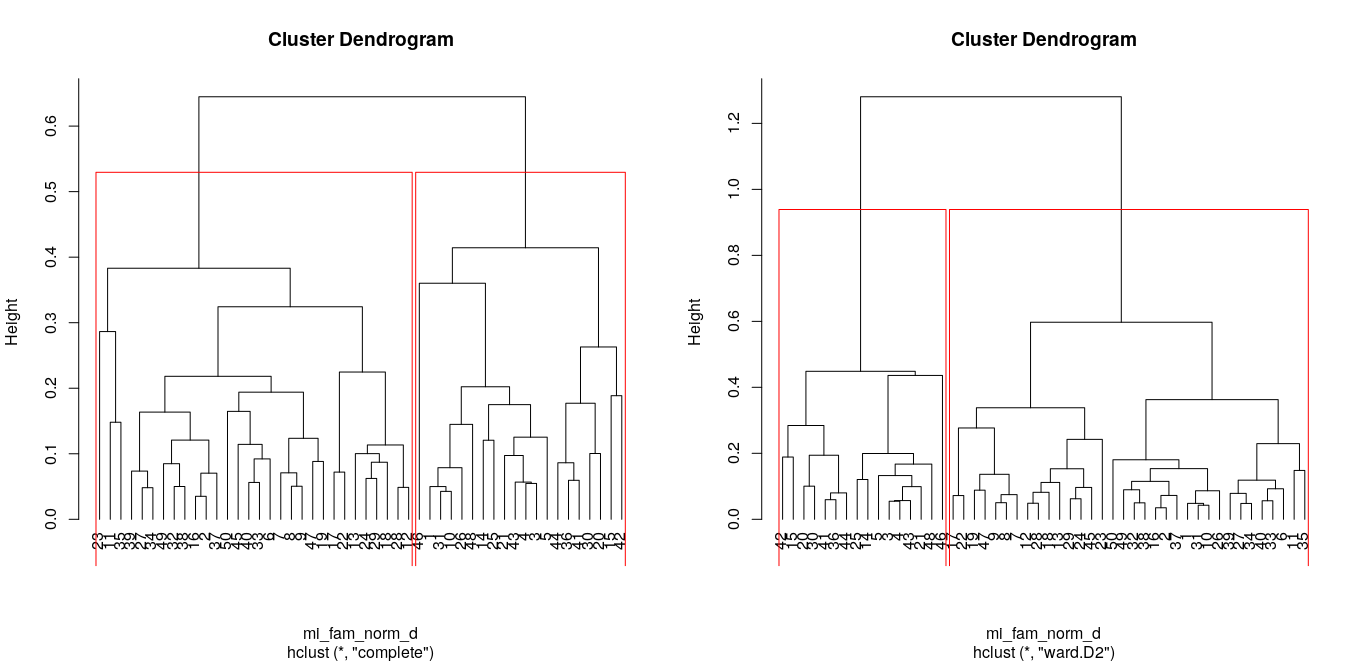
\includegraphics{grupos_ward_complete_altura_corte2.png}
\caption{Dendrogramas de los grupos producidos por Ward y Complete.
\label{fig:grupos_ward_complete_altura_corte2}}
\end{figure}

Se realizó un acercamiento restringido de la ordenación para probar el
grado de dependencia de los datos de la matriz de comunidad con la
matriz ambiental, mediante ajuste lineal en un análisis de redundancia
(RDA) (Borcard et al., 2018), utilizando la matriz de comunidad
transformada por Hellinger. Se seleccionaron las variables que
presentaron cierto grado de asociación, y (a discreción y de manera
secuencial) se excluyeron algunas de estas, con el objetivo de reducir
el grado de colinealidad entre las variables independientes restantes.

\subsection{Análisis de la
diversidad}\label{anuxe1lisis-de-la-diversidad}

Con la finalidad de asignar medidas apropiadas a la diversidad de
especies, y aprovechando su relación con los índices de Shannon y
Simpson, se empleó la serie de números de diversidad de Hill, la fórmula
de la entropía de Rengi y el índice de equidad de Pielou. Se examinó la
posible correlación entre estas medidas y las variables ambientales que
aparentaron tener algun efecto en la riqueza y equidad de la comunidad
(Borcard et al., 2018). Además, mediante interpolación por rarefacción
al número de individuos del cuadrante con la menor abundancia, se
compara el valor esperado de riqueza para todos los sitios.
Adicionalmente, se estima la riqueza de la familia Rubiaceae que
resultaría de aumentar al doble el muestreo realizado en BCI, mediante
los métodos de extrapolación incluidos en las colecciones de funciones
\texttt{SpadeR} y \texttt{iNEXT} (Chao, Ma, Hsieh, \& Chiu, 2016; Hsieh,
Ma, \& Chao, 2020), modificadas por Martínez Batlle (2020).

La variación en la composición y abundancia de especies de la comunidad,
es medida utilizando el índice multiplicativo de diversidad beta basado
en los números de Hill (Borcard et al., 2018). Finalmente, se examina la
contribución a la diversidad beta por parte de las especies y los sitios
en BCI, al analizar la varianza de la abundancia y riqueza de los
cuadrantes y las especies. Estos valores fueron comparados con la
varianza promedio, y se considera entonces que las especies cuya
varianza promedio supera la mitad de la varianza promedio total,
presentan una contribución importante a la diversidad beta de la
comunidad (Borcard et al., 2018).

\section{Resultados}\label{resultados}

La familia Rubiaceae en Barro Colorado se encuentra representada por 31
especies y 20 géneros. El género \emph{Psychotria} presenta la mayor
riqueza (8 especies). La tabla \ref{tab:abun_sp} resume las abundancias
de las especies de toda la comunidad, que en total suman 41,838
individuos, con una abundancia media de 65 individuos y mediana ubicada
en los 1,350 individuos. El gráfico de mosaicos de la figura
\ref{fig:abun_sp_q} presenta la riqueza numérica de las especies por
cuadrante. En el mismo se observa la marcada diferencia entre las
especies en cuanto a su incidencia. Además, el número de individuos de
las especies más abundantes, como \emph{Faramea occidentalis}, se
mantiene prácticamente constante en todos los cuadrantes. Por otro lado,
la abundancia de toda la comunidad muestra un aparente patrón en la
parte centro-occidental de BCI, donde se encuentran los sitios con la
mayor abundancia (ver figura \ref{fig:mapa_cuadros_abun_rubic}).

\begin{figure}
\centering
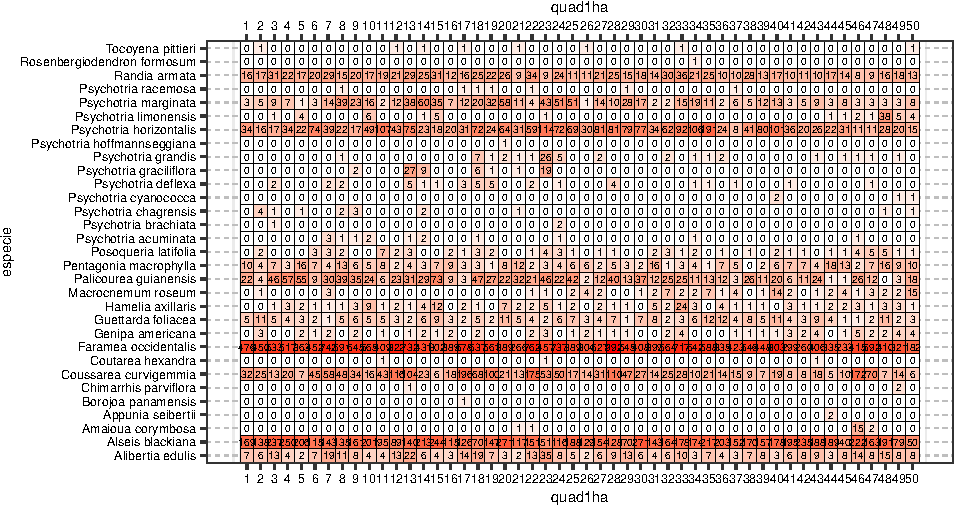
\includegraphics{manuscrito_files/figure-latex/unnamed-chunk-2-1.pdf}
\caption{\label{fig:abun_sp_q}Número de individuos de cada especie por
cuadrante.}
\end{figure}

\begin{figure}
\centering
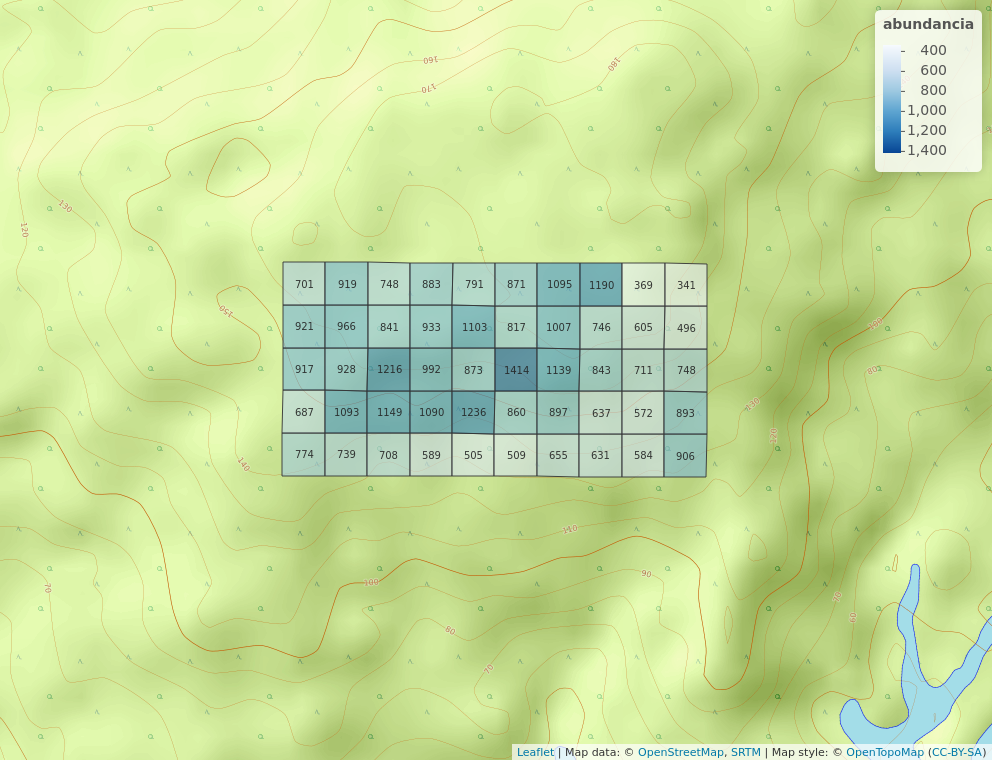
\includegraphics{mapa_cuadros_abun_rubic.png}
\caption{Abundancia de rubiaceas en BCI
\label{fig:mapa_cuadros_abun_rubic}}
\end{figure}

Los valores para el coeficiente de Spearman presentados en el panel de
correlación de la figura \ref{fig:panel_cor_suelo_abun_riq_rubic_spear},
no mostraron evidencia de que exista relación entre la riqueza y la
abundancia especies con las variables geomorfológicas notadas en la
matriz de variables ambientales. Sin embargo, el mismo análisis sugiere
una posible relación entre la abundancia numérica de especies y la
compososición del suelo, mostrando relación positiva con valores altos
de aluminio y fósforo. Así como negativa, para valores altos de pH y
concentraciones de otros elementos.

\begin{figure}
\centering
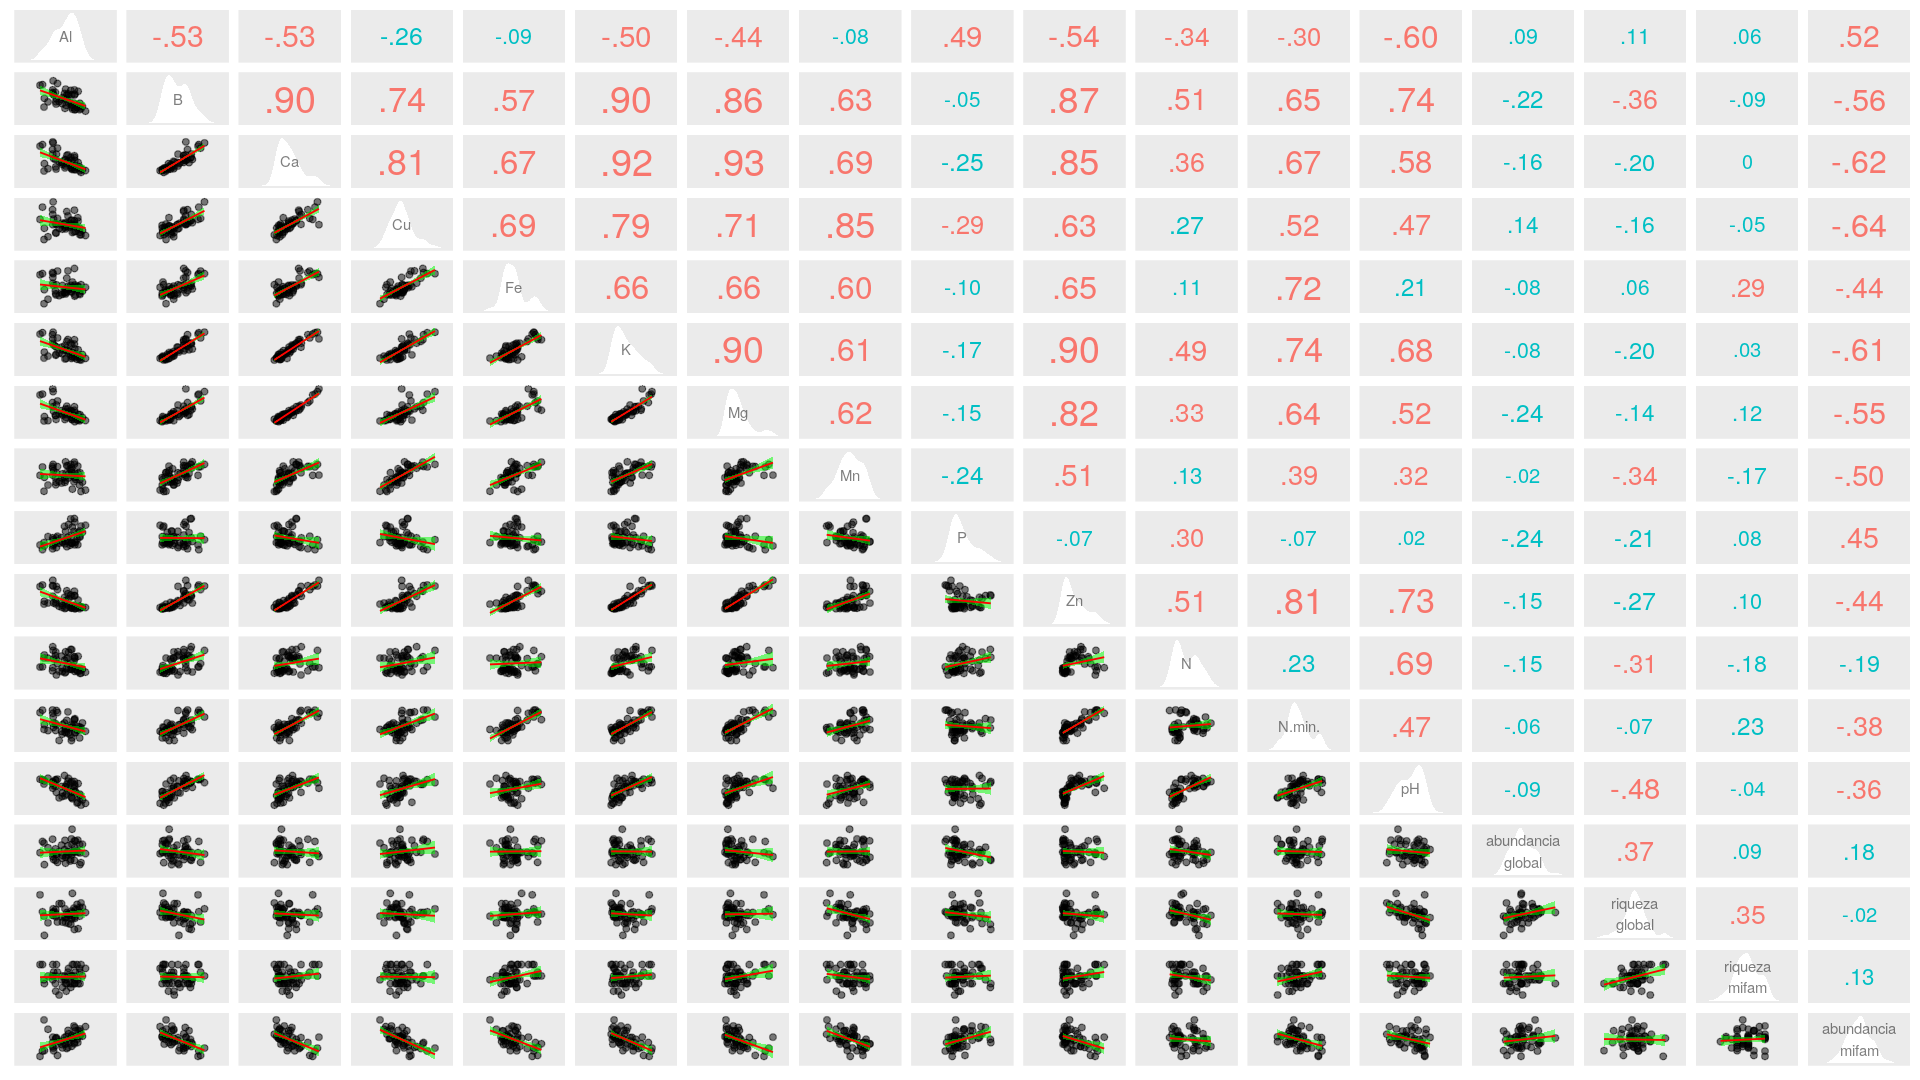
\includegraphics[width=0.80000\textwidth]{panel_cor_suelo_abun_riq_rubic_spear.png}
\caption{Panel de correlacion de Spearman entre la diversidad/abundancia
de rubiaceas y las variables edafológicas
\label{fig:panel_cor_suelo_abun_riq_rubic_spear}}
\end{figure}

Las pruebas de correlación entre los grupos 1 y 2 formulados por
complete, resultaron significativas respecto a la variable fósforo. Por
otro lado, el contenido de cobre y la abundancia global promedio, es
decir, la media correspondiente a todas las plantas en BCI, son
significativamente diferentes entre los sitios de ambos grupos, para un
nivel de significancia de \(\alpha= 0.1\) (ver
\ref{fig:diagrama_caja_igualdad_medias_complete}).

Las especies \emph{Alseis blackiana} y \emph{Psychotria limonensis}
fueron las que obtuvieron un valor alto de confianza al examinar su
potencial como especies indicadoras del grupo 1. Para el caso del grupo
2, las especies indicadoras fueron \emph{Faramea occidentalis},
\emph{Psychotria horizontalis} y \emph{Coussarea curvigemmia}. La
ocurrencia de \emph{A. blackiana} y \emph{Pentagonia macrophylla} indica
su preferencia por el grupo 1. Por otra parte, en el grupo 2 (complete)
siete especies resultan de interes por su ocurrencia: la muy dominante
\emph{F. occidentalis}; \emph{Psychotria deflexa}, \emph{P. racemosa},
\emph{P. horizontalis}, \emph{Posoqueria latifolia}, \emph{Alibertia
edulis} y \emph{Coussarea curvigemmia}. En los grupos generados mediante
Ward solo \emph{F. occidentalis}, \emph{P. horizontalis} y \emph{A.
blackiana} resultaron compatibles en las pruebas de fidelidad de
asociación.

\begin{figure}
\centering
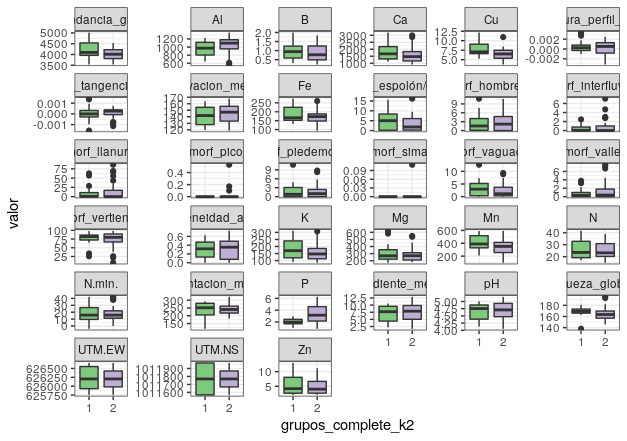
\includegraphics{diagrama_caja_igualdad_medias_complete.png}
\caption{Diagramas de caja de las variables que tuvieron un efecto,
según las pruebas de igualdad de medias. Los valores que presentan las
medianas de la variable fósforo son muy distintos entre el grupo 1
(verde) y el grupo 2 (gris).
\label{fig:diagrama_caja_igualdad_medias_complete}}
\end{figure}

En el diagrama rotulado como escalamiento 1 de la figura
\ref{fig:pca_biplot_suelo}, se observan tres grupos de cuadrantes
diferenciados entre sí. Un grupo de sitios con un alto grado de acidez y
contenido en aluminio, otro grupo caracterizado por la presencia de
elementos metálicos, y un tercero, con una cantidad de fósforo,
nitrógeno y valor de pH mayor. En el caso de las variables
geomorfológicas, algunos sitios están asociados a un alto porcentaje de
llanura y hombrera, aunque la mayoría se encuentra más cerca del origen
formado por los ejes de los componentes principales 1 y 2 (ver figura
\ref{fig:pca_biplot_geomorf}).

Los resultados del PCA de los datos de la matriz de comunidad se
encuentran resumidos en los diagramas de la figura
\ref{fig:pca_biplot_sps}. El escalamiento 1, muestra muchos de los
cuadrantes dispuestos alrededor del origen formado por los ejes, lo que
indica una contribución a la varianza relativamente equitativa por parte
de las especies. Sin embargo, aparecen también unos cuantos cuadrantes
con valores atípicos y más alejados. Se nota como las especies \emph{A.
blackiana}, \emph{C. curvigemmia}, \emph{P. marginalis} y \emph{P.
horizontalis}, presentan una contribución desproporcionada a la varianza
total, en comparación con el resto de las especies.

El escalamiento 2 de la figura
\ref{fig:biplot_correspndncia_sps_escal_2_2} en el análisis de
correspondencia mostró que las especies \emph{Psychotria graciliflora} y
\emph{Psychotria grandis} se encuentran asociadas. Ambas especies,
además, tienen valores de abundancia parecidos dentro de la comunidad
(65 y 57 individuos, respectivamente). Casi todas las demás especies se
encuentran próximas al punto de intersección, salvo aquellas que
presentaron una abundancia reducida, y en consecuencia aparecen cercanas
a los pocos cuadrantes en los que se encuentran mejor representadas. La
disparidad en la incidencia de las especies se refleja en su disposición
en el diagrama. Sin embargo, estos resultados no coinciden del todo con
los arrojados por el PCA de la matriz de distancias Hellinger.

\begin{figure}
\centering
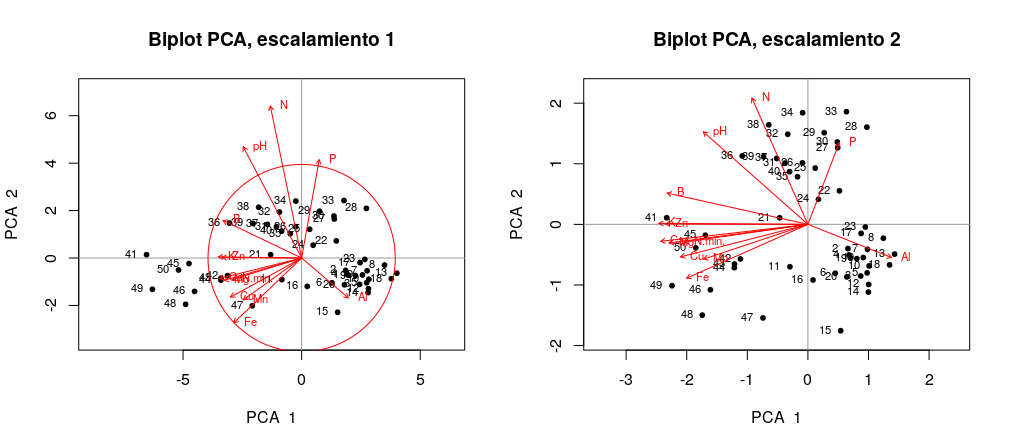
\includegraphics{pca_biplot_suelo.png}
\caption{Biplots generados en el PCA de las variables de suelo. Se
observa que las variables nitrógeno, fósforo y pH aportan la mayor parte
de la varianza explicada. La relación entre las variables se encuentra
debidamente representada en el recuadro del escalamiento 2, por medio de
los ángulos que forman sus vectores. \label{fig:pca_biplot_suelo}}
\end{figure}

\begin{figure}
\centering
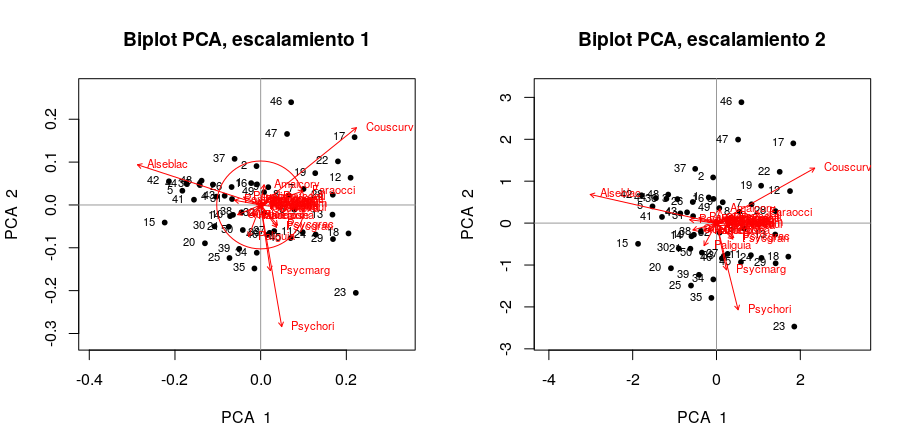
\includegraphics{pca_biplot_sps.png}
\caption{Biplots producidos por PCA de los datos de comunidad
transformados a distancias Hellinger. \label{fig:pca_biplot_sps}}
\end{figure}

\begin{figure}
\centering
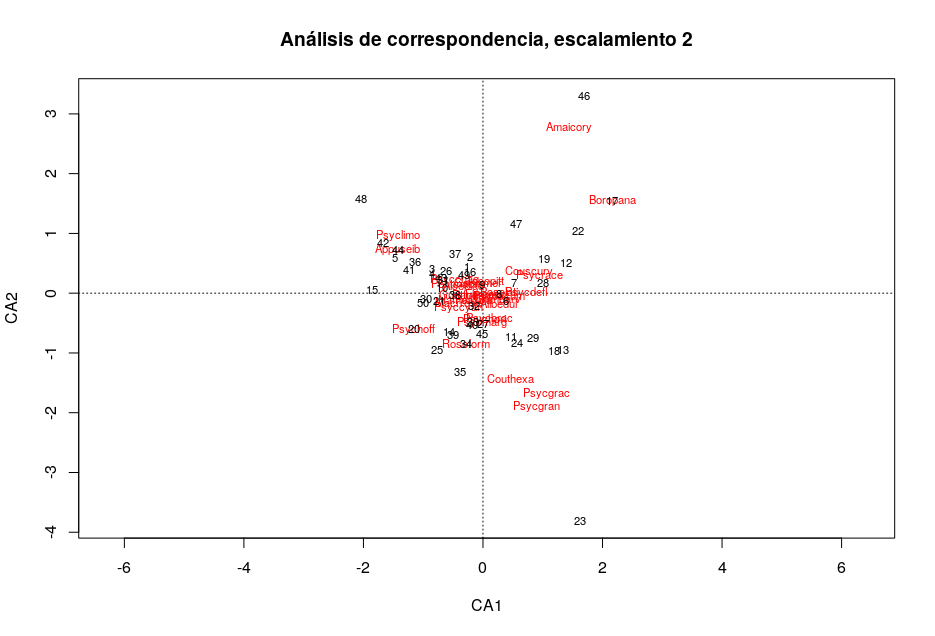
\includegraphics{biplot_correspndncia_sps_escal_2_2.png}
\caption{Biplot del análisis de correspondencia de los datos de
abundancia de las especies de Rubiaceae.
\label{fig:biplot_correspndncia_sps_escal_2_2}}
\end{figure}

Se observa asociación entre el contenido de cobre, manganeso y fósforo
con algunos sitios y especies, en el \emph{biplot} del análisis de
coordenadas principales de la figura
\ref{fig:pcoa_sps_jacc_var_ambient}. También, algunas de las especies
menos abundantes de la comunidad se presentan asociadas a algunos sitios
comunes entre las mismas. Es probable que esta aparente asociación
aparezca debido a la combinación de una incidencia restringida por parte
de estas especies y al alto grado de autocorrelación entre los
cuadrantes.

\begin{figure}
\centering
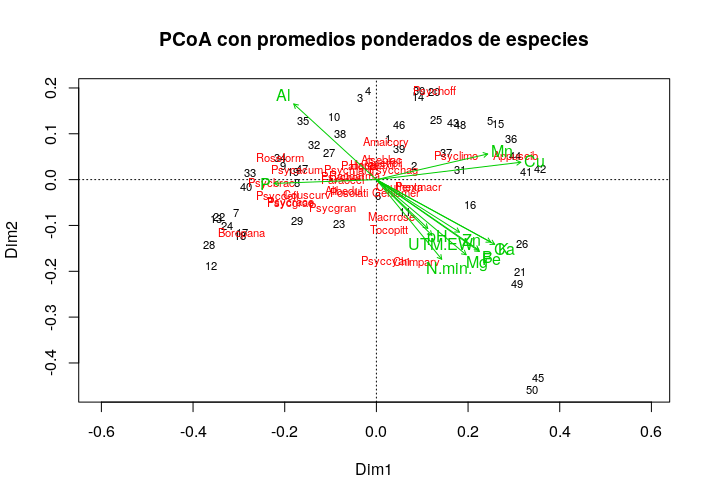
\includegraphics{pcoa_sps_jacc_var_ambient.png}
\caption{Biplot de PCoA de las distancias de Jaccard. Las distancias
entre especies están ponderadas en base a sus valores de abundancia.
\label{fig:pcoa_sps_jacc_var_ambient}}
\end{figure}

\section{RDA}\label{rda}

Se destacan los patrones encontrados en los resultados encontrados por
las pruebas de asociación y los arrojados por el análisis de
redundancia. En los \emph{triplots} producidos por RDA (figura
\ref{fig:rda_triplot_var_selec_4_escal2}), los vectores representando
los datos de las especies se disponen en forma de abanico

En cuanto a los \emph{triplots} generados por RDA mostrados en la se
destacan los la distancia euclídea conservada entre las especies. Estas
últimas se disponen en ¿ algunas resultan aberraciones, muy alejadas del
punto de intercepto, sitios emjambrados en el origen, y las especies
dispuestas en forma de abanico a su alrededor. Esto indica poca
asociación entre las especies, no se encuentra un patrón evidente entre
la mayoría. Se destaca un grupo de cuadrantes en los cuales
\emph{Psychotria horizontalis} y \emph{Psychotria marginata} se
encuentran asociadas. Al parecer, este grupo de cuadrantes constituye un
microhabitat encontrado sobre una pequeña meseta en la parte
nor-oriental de BCI, y se diferencia además por una alta concentración
de fósforo y aluminio en el suelo. La especie \emph{Alseis blackiana}
presenta asociación con el contenido de metales como manganeso, hierro y
cobre en el suelo, esto coincide con los resultados del PCA, y podría
ser considerada como una especie indicadora de estas condiciones
ambientales.

\begin{figure}
\centering
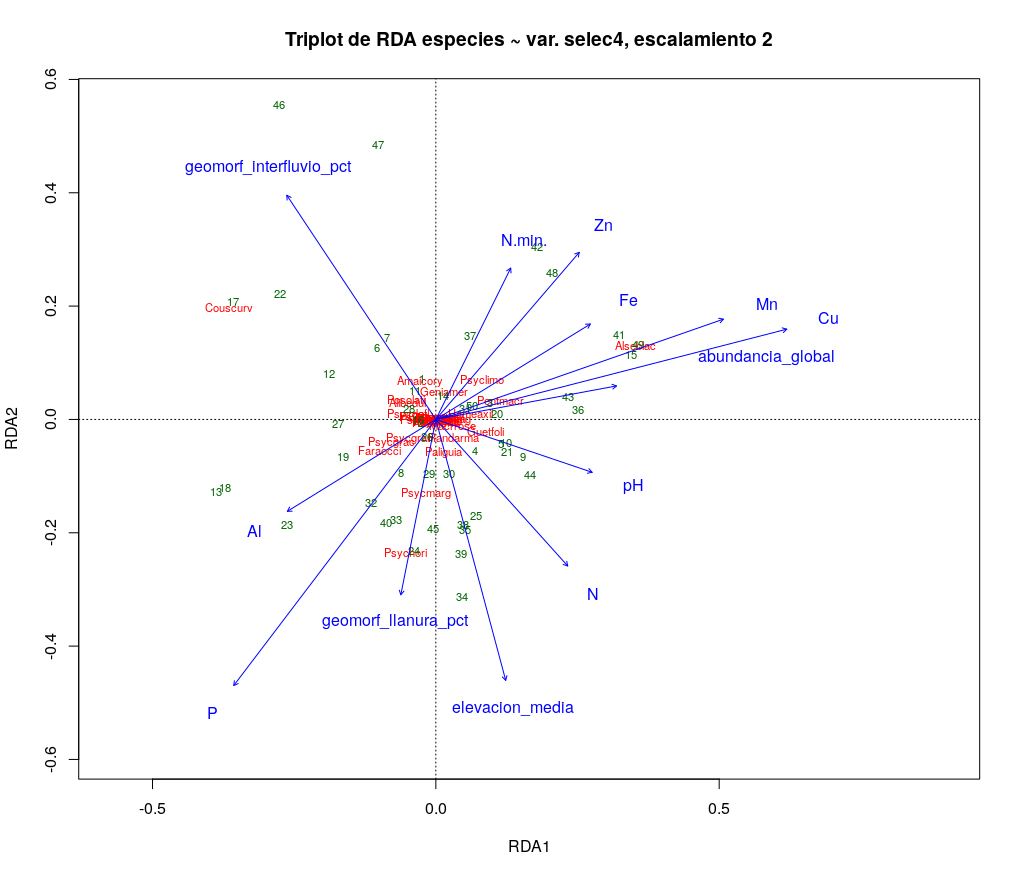
\includegraphics{rda_triplot_var_selec_4_escal2.png}
\caption{Triplot del RDA de los valores de abundancia transformados. Las
variables ambientales que se observan fueron las seleccionadas para
restringir la varianza explicada de los datos de comunidad.
\label{fig:rda_triplot_var_selec_4_escal2}}
\end{figure}

\section{Diversidad}\label{diversidad}

La riqueza de la familia aumenta con el hierro, así tambien la equidad.
Además, parece que la riqueza aumenta en los suelos con un alto
contenido de nitrógeno en el suelo y en su forma mineralizada. La
equidad también es mayor hacia el norte de bci
{[}\ref{fig:panel_cor_indics_diversidad1_columnnas_quitadas}{]}.

 \ref{fig:rarefaccion_min_abun}

Sitio 1 con la menor riqueza presenta una de las mayores dominancias.
También el sitio 28 aunque no tanto por el número de especies
presentado, sino más bien por su desorbitada abundancia (1414 indiv.) .
50 con la menor abundancia.

Aparte del cuadrante 50, los sitios con la mayor riqueza presentan
también mucha abundancia. las especies dominantes están adaptadas a
reclutar nuevos individuos con y sin interferencia de otras especies?
Las especies menos abundantes están adaptadas a vivir apretujadas? Es
todo esto casualidad?

Las especies que contribuyen de manera significativa a la diversidad
beta. Muchas de estas especies fueron consideradas ``indicadoras''
debido a su abundancia. Con la excepción de la especie \emph{Macocnemum
roseum}, la cual presenta una abundancia mucho menor a la de las demás
especies que resultan de este análisis.

Alseis blackiana Coussarea curvigemmia Faramea occidentalis Macrocnemum
roseum Palicourea guianensis 0.18474561 0.15378542 0.05287862 0.03793339
0.09128798 Pentagonia macrophylla Psychotria horizontalis Psychotria
limonensis Psychotria marginata 0.03945305 0.11389433 0.03848514
0.08084602

\begin{figure}
\centering
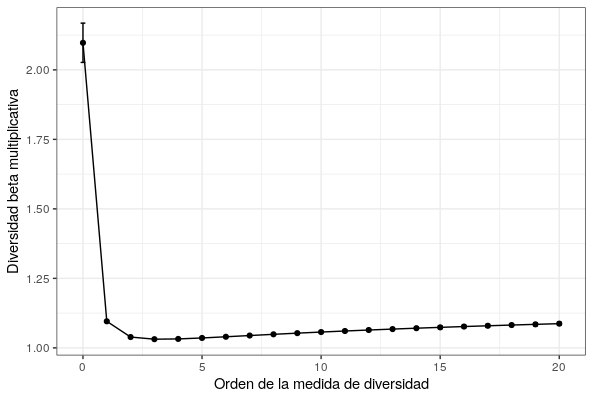
\includegraphics{grafico_divrsdad_beta_hill.png}
\caption{Gráfico de la diversidad beta multiplicativa en función de los
números en la serie de Hill. Se observa que la riqueza de especies
(número de Hill 0) presenta la mayor contribución a la medida de
diversidad beta para la comunidad. Así sucede ya que la abundancia de
las especies dominantes no varía drásticamente entre cuadrantes, y es
principalmente su composición de especies lo que diferencia a los sitios
entre sí. \label{fig:grafico_divrsdad_beta_hill}}
\end{figure}

El grado de reemplazo o diversidad beta entre\ldots{}. se midió
utilizando del índice multiplicativo de diversidad beta aplicando

el comportamiento de la dominancia que siguen las especies de la
comunidad---- en cuanto a la dominancia de las especies

La representatibidad de la parcela permanente comparada con el valor
posible real de la riqueza de esta familia a nivel local?

Estimar la riqueza que se conseguiría con más parcelas de censo en BCI?

El grupo 2 (1 en Ward) contiene los sitios con tendencia a presentar
valores altos de acidez {[}\ref{fig:mapa_cuadros_ph}{]} y concentración
de aluminio.

\begin{figure}
\centering
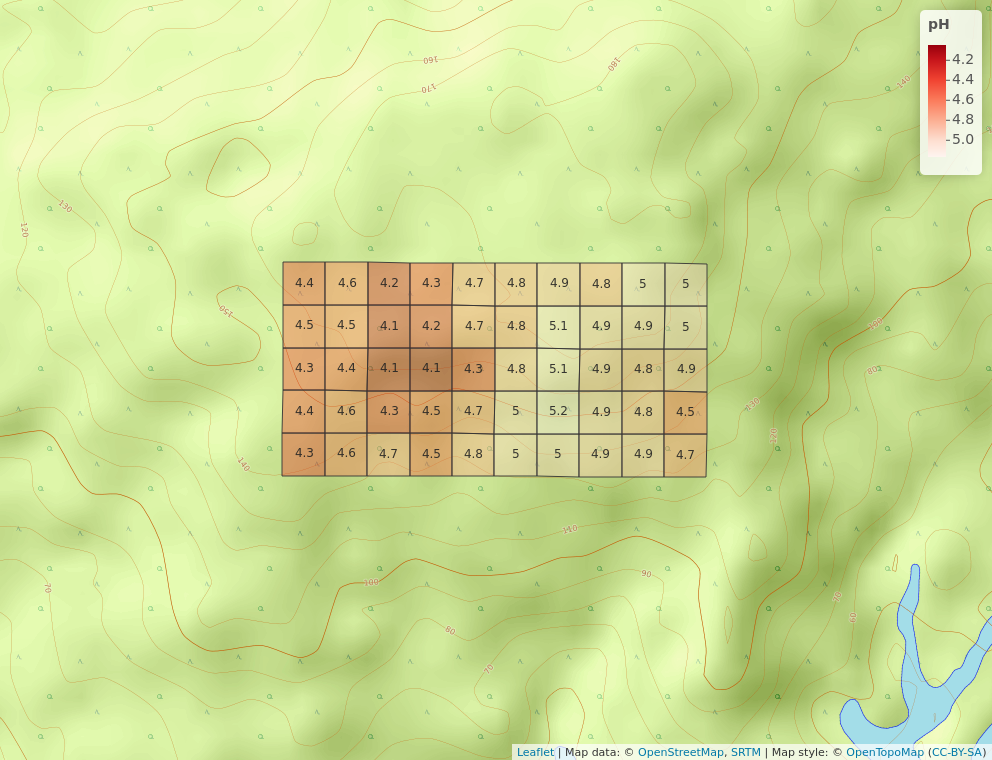
\includegraphics{mapa_cuadros_ph.png}
\caption{pH del suelo en los cuadros de 1ha \label{fig:mapa_cuadros_ph}}
\end{figure}

\begin{figure}
\centering
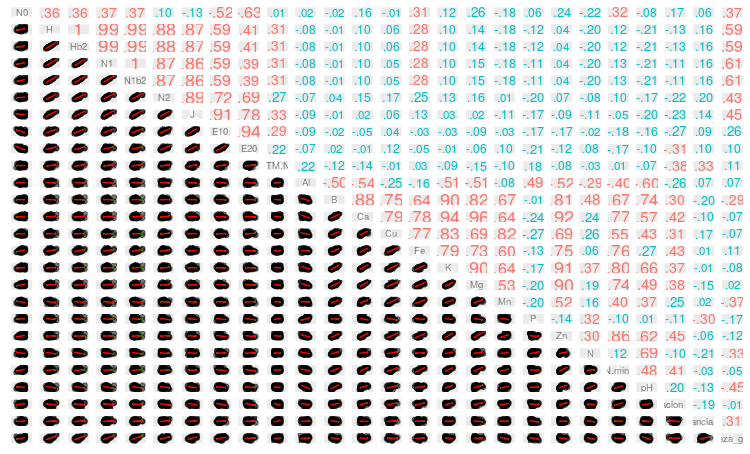
\includegraphics{panel_cor_indcs_diversidad1_columnas_quitadas.png}
\caption{Correlación entre diversidad/equidad y algunas de las variables
ambientales destacadas. \(N0\): riqueza de especies; \(H\): entropía de
Shannon; \(Hb2\): entropía de Shannon con 2 como base del logaritmo;
\(N1\) y \(N2\): Números de Hill; \(N1b2\): Número de Hill 1 en base log
2; \(J\): Equidad de Pielou; \(E10\) y \(E20\): ratios de Hill 1 y 2.
\label{fig:panel_cor_indics_diversidad1_columnnas_quitadas}}
\end{figure}

\begin{figure}
\centering
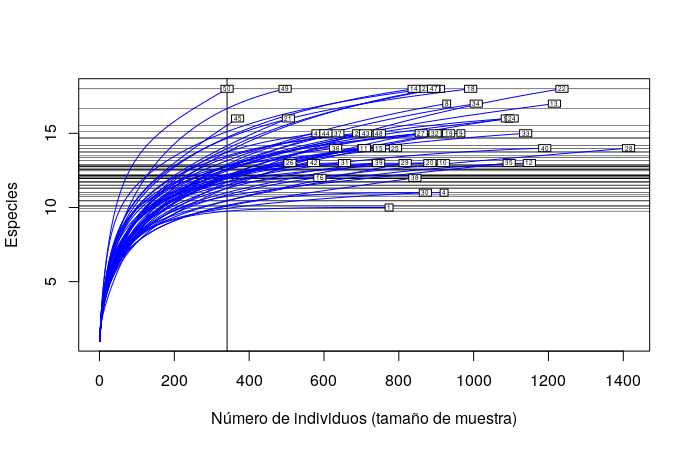
\includegraphics{rarefaccion_min_abun.png}
\caption{Curva de rarefacción. Las barras horizontales muestran el valor
de la riqueza esperada en cada sitio al interpolar las muestras hacia la
abundancia mínima observada (341 individuos), presente en el cuadrante
\#50. \label{fig:rarefaccion_min_abun}}
\end{figure}

\begin{figure}
\centering
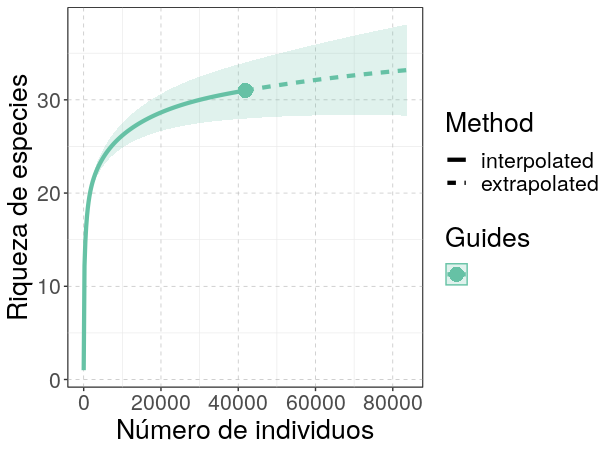
\includegraphics{curva_extrapol_doble_esfuerzo.png}
\caption{Curva de acumulación de especies hacia el doble de la
abundancia encontrada en BCI. Se estima que la riqueza aumentaría en
cuatro especies en consecuencia de duplicar el senso, o replicarlo en
otra zona de Barro Colorado. El intervalo para un 95\% de confianza se
representa con los márgenes verde pálido.
\label{fig:curva_extrapol_doble_esfuerzo}}
\end{figure}

\section{Discusión}\label{discusiuxf3n}

La determinación de las especies indicadoras \emph{Faramea occidentalis}
y \emph{Alseis blackiana} de los grupos uno y dos podría estár asociada
a la evidente dominancia que presentan estas especies en la comunidad de
rubiaceas. Especialmente \emph{F. occidentalis}, cuya abundancia alcanza
valores extremos dentro de todo BCI e incluso podría estar inclinando
los resultados de estos analisis?. Esto se vuelve razonable al tomarse
en cuenta el hecho de que muchas especies se presentaban con pocos
valores de abundancia, varias incluso representadas por un solo
individuo. Las especies con preferencia por el grupo 1 evaden
sistemáticamente al grupo 2 y viceversa. Esta diferenciación en la
ocurrencia de las especies no se explica del todo con las variables
ambientales medidas en BCI y es posible que exista algun otro factor que
determina la ordenación de esta comunidad de plantas. La cobertura del
dosel arbóreo podría ser una de estas variables a considerarse, puesto
que las especies dominantes en la comunidad son a la vez tolerantes a la
sombra (Grandtner \& Chevrette, 2013). la relación entre la abundancia
de la familia y el contenido de alumínio y fósforo. Esto coincidió con
los análisis de la varianza explicada entre variables, aunque solo para
la concentración de fósforo. Adicionalmente, la comunidad de rubiaceas
pareciera poder dividirse en dos grupos relativamente bien diferenciados
entre sí por sus diferencias en el contenido de \emph{Cu} y \emph{P} del
suelo. . Es probable que las especies indicadoras del grupo con un mayor
contenido de cobre estén mostrando preferencia por estas condiciones
ambientales. Sin embargo, el pH y la mayoría de componentes del suele en
BCI tienen valores bastante homogéneos y más bien se presentan pequeños
gradientes entre algunos lugares, lo cual evita que este tipo de
acercamiento sea concluyente.

Algunas de las pruebas estadísticas empleadas en este estudio requieren
del supuesto de independencia entre muestras, supuesto que es incumplido
por los cuadrantes en BCI debido a su contigüidad. Sin embargo, esta
condición permitió un acercamiento comparativo con las técnicas
apropiadas para el análisis de muestras con cierto grado asociación
entre sí. En BCI, tanto las variables ambientales como las comunidades
de plantas se encuentran correlacionadas espacialmente. Por lo tanto,
los patrones encontrados entre métodos contrastados son cuanto menos
interesantes. El área correspondiente a BCI es bastante homogénea en
cuanto a sus condiciones físicas, ya que fué diseñada para que así fuera
(Baillie, Elsenbeer, Barthold, Grimm, \& Stallard, 2006). Como la misma
se encuentra situada sobre el dorso de una cuesta de andesita, las
variables edafológicas aquí presentes en su mayoría siguen un gradiente
a lo largo de todo BCI, resultado de la meteorización de la roca
original (Patino, Velbel, Price, \& Wade, 2003).

Los análisis de agrupamiento pueden verse sesgados por la heterogeneidad
morfométrica que pueden presentar las plantas de esta familia. Estas
especies presentan diversos hábitos de crecimiento, desde porte herbáceo
y arbustivo a árboles relativamente grandes. Esto hace que el hecho de
que se incluya el criterio de dap de 10 mm en el momento de ser censadas
podría estar excluyendo especies clave en el rompecabezas.

\section{Agradecimientos}\label{agradecimientos}

\section{Información de soporte}\label{informaciuxf3n-de-soporte}

\begin{longtable}[]{@{}lr@{}}
\caption{\label{tab:abun_sp}Abundancia total por
especie.}\tabularnewline
\toprule
Latin & n\tabularnewline
\midrule
\endfirsthead
\toprule
Latin & n\tabularnewline
\midrule
\endhead
Faramea occidentalis & 24989\tabularnewline
Alseis blackiana & 7928\tabularnewline
Psychotria horizontalis & 2453\tabularnewline
Coussarea curvigemmia & 2010\tabularnewline
Palicourea guianensis & 1118\tabularnewline
Randia armata & 937\tabularnewline
Psychotria marginata & 761\tabularnewline
Alibertia edulis & 417\tabularnewline
Pentagonia macrophylla & 306\tabularnewline
Guettarda foliacea & 252\tabularnewline
Hamelia axillaris & 128\tabularnewline
Macrocnemum roseum & 87\tabularnewline
Posoqueria latifolia & 73\tabularnewline
Psychotria limonensis & 70\tabularnewline
Genipa americana & 67\tabularnewline
Psychotria graciliflora & 65\tabularnewline
Psychotria grandis & 57\tabularnewline
Psychotria deflexa & 38\tabularnewline
Amaioua corymbosa & 19\tabularnewline
Psychotria chagrensis & 16\tabularnewline
Psychotria acuminata & 14\tabularnewline
Tocoyena pittieri & 8\tabularnewline
Psychotria racemosa & 7\tabularnewline
Psychotria cyanococca & 4\tabularnewline
Chimarrhis parviflora & 3\tabularnewline
Coutarea hexandra & 3\tabularnewline
Psychotria brachiata & 3\tabularnewline
Appunia seibertii & 2\tabularnewline
Borojoa panamensis & 1\tabularnewline
Psychotria hoffmannseggiana & 1\tabularnewline
Rosenbergiodendron formosum & 1\tabularnewline
\bottomrule
\end{longtable}

\begin{figure}
\centering
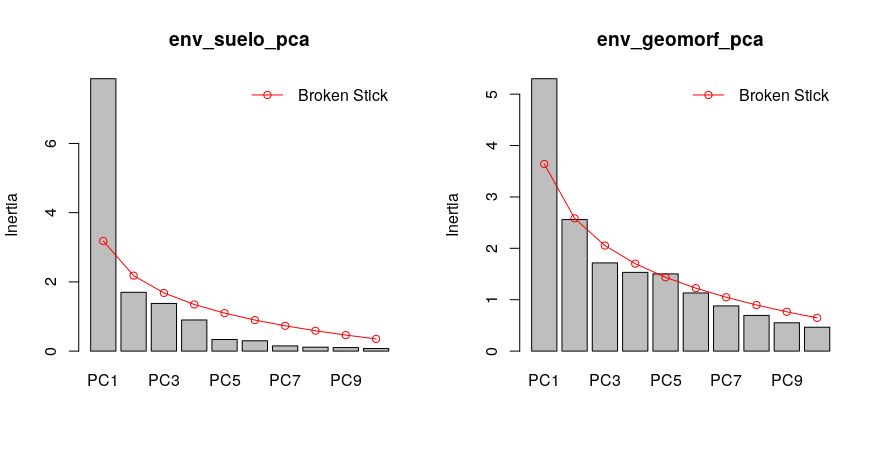
\includegraphics{env_suelo_geomorf_pca_br_stick.png}
\caption{Componentes príncipales de la varianza en las variables de
suelo y geomorfología en BCI. En estos gráficos se incluye el
comportamiento de la varianza explicada, predecido por el modelo de bara
quebrada, representado por la línea roja formando la curva. (La escala
denominada ``\emph{Inertia}'' representa la suma de los cuadrados de
toda la varianza). \label{fig:pca_suelo_geomorf_br_stick}}
\end{figure}

\begin{figure}
\centering
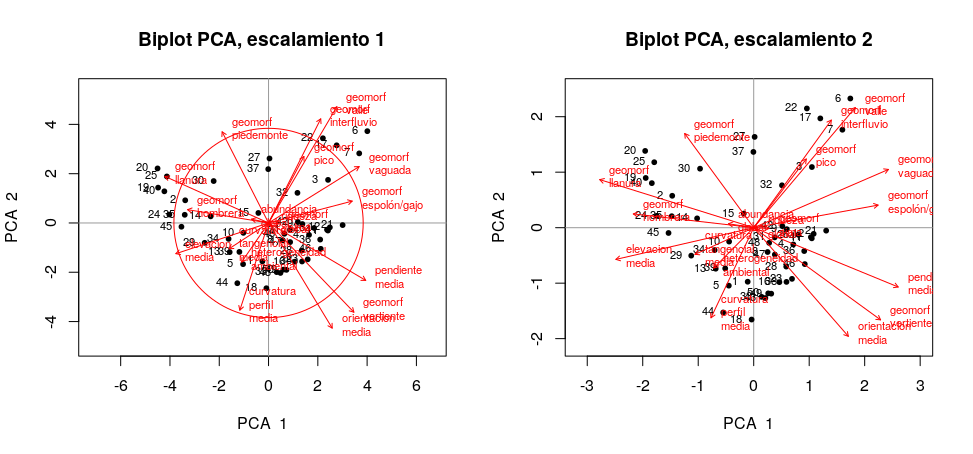
\includegraphics{pca_biplot_geomorf.png}
\caption{Biplots generados por PCA de las variables geomorfológicas.
\label{fig:pca_biplot_geomorf}}
\end{figure}

\section{\texorpdfstring{\emph{Script}
reproducible}{Script reproducible}}\label{script-reproducible}

\ldots

\section*{Referencias}\label{referencias}
\addcontentsline{toc}{section}{Referencias}

\hypertarget{refs}{}
\hypertarget{ref-cita_mapview}{}
Appelhans, T., Detsch, F., Reudenbach, C., \& Woellauer, S. (2019).
\emph{Mapview: Interactive viewing of spatial data in r}. Retrieved from
\url{https://CRAN.R-project.org/package=mapview}

\hypertarget{ref-baillie_soil}{}
Baillie, I., Elsenbeer, H., Barthold, F., Grimm, R., \& Stallard, R.
(2006). \emph{Semi-detailed soil survey of barro colorado island,
panama}.

\hypertarget{ref-borcard_legendre}{}
Borcard, D., Gillet, F., \& Legendre, P. (2018). \emph{Numerical Ecology
with R. Second Edition} (pp. 52--66).
\url{https://doi.org/10.1007/978-3-319-71404-2}

\hypertarget{ref-caceres2009associations}{}
Cáceres, M. D., \& Legendre, P. (2009). Associations between species and
groups of sites: Indices and statistical inference. \emph{Ecology},
\emph{90}(12), 3566--3574.

\hypertarget{ref-spader_chao}{}
Chao, A., Ma, K. H., Hsieh, T. C., \& Chiu, C.-H. (2016). \emph{SpadeR:
Species-richness prediction and diversity estimation with r}. Retrieved
from \url{https://CRAN.R-project.org/package=SpadeR}

\hypertarget{ref-condit_et_al_2012}{}
Condit, R., Chisholm, R. A., \& Hubbell, S. P. (2012). Thirty years of
forest census at Barro Colorado and the importance of immigration in
maintaining diversity. \emph{PLOS ONE}, \emph{7}(11), 1--6.
\url{https://doi.org/10.1371/journal.pone.0049826}

\hypertarget{ref-condit_et_al_2017}{}
Condit, R., Pérez, R., Lao, S., Aguilar, S., \& Hubbell, S. P. (2017).
Demographic trends and climate over 35 years in the Barro Colorado 50 ha
plot. \emph{Forest Ecosystems}, \emph{4}(1), 17.
\url{https://doi.org/10.1186/s40663-017-0103-1}

\hypertarget{ref-article_condit}{}
Condit, R., Pitman, N., Leigh, E., Chave, J., Terborgh, J., Foster, R.,
\ldots{} Hubbell, S. (2002). Beta-diversity in tropical forest trees.
\emph{Science (New York, N.Y.)}, \emph{295}, 666--669.
\url{https://doi.org/10.1126/science.1066854}

\hypertarget{ref-davis2009global}{}
Davis, A. P., Govaerts, R., Bridson, D. M., Ruhsam, M., Moat, J., \&
Brummitt, N. A. (2009). A global assessment of distribution, diversity,
endemism, and taxonomic effort in the rubiaceae1. \emph{Annals of the
Missouri Botanical Garden}, \emph{96}(1), 68--78.

\hypertarget{ref-cita_indicspecies}{}
De Caceres, M., \& Legendre, P. (2009). Associations between species and
groups of sites: Indices and statistical inference. In \emph{Ecology}.
Retrieved from \url{http://sites.google.com/site/miqueldecaceres/}

\hypertarget{ref-dufrene_legendre}{}
Dufrene, M., \& Legendre, P. (1997). Species assemblages and indicator
species: The need for a flexible asymmetrical approach. \emph{Ecological
Monographs}, \emph{67}, 345--366. \url{https://doi.org/10.2307/2963459}

\hypertarget{ref-grandtner2013dictionary}{}
Grandtner, M., \& Chevrette, J. (2013). \emph{Dictionary of trees,
volume 2: South america: Nomenclature, taxonomy and ecology}. Retrieved
from \url{https://books.google.com.do/books?id=XALRl1qzcLMC}

\hypertarget{ref-inext_chao}{}
Hsieh, T. C., Ma, K. H., \& Chao, A. (2020). \emph{INEXT: Interpolation
and extrapolation for species diversity}. Retrieved from
\url{http://chao.stat.nthu.edu.tw/wordpress/software_download/}

\hypertarget{ref-hubell_foster_1983}{}
Hubbell, S. P., \& Foster, R. B. (1983). Diversity of canopy trees in a
neotropical forest and implications for conservation. In T. Whitmore, A.
Chadwick, \& A. Sutton (Eds.), \emph{Tropical rain forest: Ecology and
management} (pp. 25--41). Oxford: The British Ecological Society.

\hypertarget{ref-hubell_et_all_1990}{}
Hubbell, S. P., Condit, R., Foster, R. B., Grubb, P. J., Thomas, C. D.,
Hassell, M. P., \& May, R. M. (1990). Presence and absence of density
dependence in a neotropical tree community. \emph{Philosophical
Transactions of the Royal Society of London. Series B: Biological
Sciences}, \emph{330}(1257), 269--281.
\url{https://doi.org/10.1098/rstb.1990.0198}

\hypertarget{ref-web_bci}{}
Hubbell, S., Condit, R., \& Foster, R. (2021). Forest Census Plot on
Barro Colorado Island. Retrieved March 23, 2021, from
\url{http://ctfs.si.edu/webatlas/datasets/bci/}

\hypertarget{ref-article}{}
Jansen, S., Robbrecht, E., Beeckman, H., \& Smets, E. (2000). Aluminium
accumulation in rubiaceae: An additional character for the delimitation
of the subfamily rubioideae? \emph{IAWA Journal}, \emph{21}.
\url{https://doi.org/10.1163/22941932-90000245}

\hypertarget{ref-legendre_galllagher_2001}{}
Legendre, P., \& Gallagher, E. (2001). Ecologically meaningful
transformations for ordination of species data. \emph{Oecologia},
\emph{129}, 271--280. \url{https://doi.org/10.1007/s004420100716}

\hypertarget{ref-jose_ramon_martinez_batlle_2020_4402362}{}
Martínez Batlle, J. R. (2020).
biogeografia-master/scripts-de-analisis-BCI: Long coding sessions
(Version v0.0.0.9000). \url{https://doi.org/10.5281/zenodo.4402362}

\hypertarget{ref-moreno2001manual}{}
Moreno, C. E. (2001). \emph{Manual de métodos para medir la
biodiversidad}. Universidad Veracruzana.

\hypertarget{ref-2008arXiv0803.3704N}{}
Néda, Z., Horvat, S., Toháti, H. M., Derzsi, A., \& Balogh, A. (2008). A
spatially explicit model for tropical tree diversity patterns.
\emph{arXiv E-Prints}, arXiv:0803.3704.

\hypertarget{ref-cita_vegan}{}
Oksanen, J., Blanchet, F. G., Friendly, M., Kindt, R., Legendre, P.,
McGlinn, D., \ldots{} Wagner, H. (2019). \emph{Vegan: Community ecology
package}. Retrieved from \url{https://CRAN.R-project.org/package=vegan}

\hypertarget{ref-patino_weathering}{}
Patino, L., Velbel, M., Price, J., \& Wade, J. (2003). Trace element
mobility during spheroidal weathering of basalts and andesites in hawaii
and guatemala. \emph{Chemical Geology}, \emph{202}.
\url{https://doi.org/10.1016/j.chemgeo.2003.01.002}

\hypertarget{ref-cita_sf}{}
Pebesma, E. (2018). Simple Features for R: Standardized Support for
Spatial Vector Data. \emph{The R Journal}, \emph{10}(1), 439--446.
\url{https://doi.org/10.32614/RJ-2018-009}

\hypertarget{ref-cita_r}{}
R Core Team. (2020). \emph{R: A language and environment for statistical
computing}. Retrieved from \url{https://www.R-project.org/}

\hypertarget{ref-TORRESLEITE2019151487}{}
Torres-Leite, F., Cavatte, P. C., Garbin, M. L., Hollunder, R. K.,
Ferreira-Santos, K., Capetine, T. B., \ldots{} Carrijo, T. T. (2019).
Surviving in the shadows: Light responses of co-occurring rubiaceae
species within a tropical forest understory. \emph{Flora}, \emph{261},
151487.
\url{https://doi.org/https://doi.org/10.1016/j.flora.2019.151487}

\hypertarget{ref-Volkov_2003}{}
Volkov, I., Banavar, J. R., Hubbell, S. P., \& Maritan, A. (2003).
Neutral theory and relative species abundance in ecology. \emph{Nature},
\emph{424}(6952), 1035--1037. \url{https://doi.org/10.1038/nature01883}

\hypertarget{ref-cita_tidyverse}{}
Wickham, H. (2017). \emph{Tidyverse: Easily install and load the
'tidyverse'}. Retrieved from
\url{https://CRAN.R-project.org/package=tidyverse}




\newpage
\singlespacing 
\end{document}
